\section{Soft artificial life: substrates and evolutionary mechanisms}
Figure~\ref{fig:substrates} distinguishes the local transition units before
comparing their reproductive or evolutionary capabilities.
\begin{figure}[!htbp]
\centering
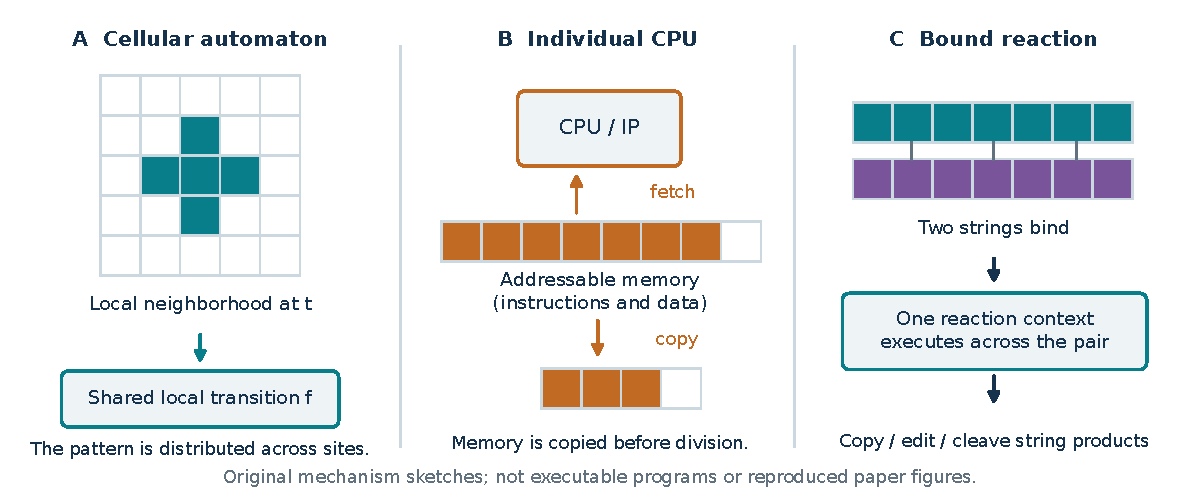
\includegraphics[width=\textwidth]{figures/soft-substrates.pdf}
\caption{Three computational substrates, drawn as original mechanism sketches
from the descriptions of cellular automata, Tierra, and spatial Stringmol
\citep{Langton1984,Ray1991,Hickinbotham2021}. The highlighted CA neighborhood is
not a reproducing loop. Tierra separates CPU ownership from code location;
Stringmol executes through a bound-pair reaction context. The panels do not
assert equivalent reproduction or evolutionary capabilities.}
\label{fig:substrates}
\end{figure}
\subsection{Discrete cellular automata and construction}
A cellular automaton specifies a spatial state and a local transition, commonly
written schematically as
\begin{equation}
 x_i(t+1)=f\!\left(x_j(t):j\in\mathcal N(i)\right).
\end{equation}
The neighborhood, boundary conditions, state alphabet, and update schedule are
parts of the model. Simple local descriptions can support elaborate structures,
but visual elaboration alone does not identify reproduction or heredity.

Langton's engineered self-reproducing loop demonstrates that a compact local
construction process need not be a universal constructor
\citep{Langton1984}. Its circulating information participates in constructing
and copying a new loop. The result concerns an explicit reproduction mechanism;
it does not establish spontaneous origins or indefinitely diversifying
descendants. Evoloops add an instructive contrast: interaction and collision
under deterministic rules can alter reproducing structures and generate
inherited variation \citep{Sayama1998,SayamaNehaniv2024}. Reported size
convergence also shows why an evolving population is not sufficient evidence
of ongoing novelty.

These systems make a central point for kernel design. Variation need not always
be an externally sampled mutation event: it can result from ordinary
interactions in the substrate. Conversely, declaring a rule local does not
make its consequences unstructured by design. The state alphabet and
transition table already determine which constructions are possible.

\subsection{Executable digital organisms: Tierra and Avida}
Executable-genome systems place variation inside programs whose operations
affect their own continuation. Tierra uses a shared memory environment and
individual execution contexts; allocation, copying, and division participate
in reproduction \citep{Ray1991}. Execution ownership and code location are
distinct: an individual's CPU can execute another individual's instructions.
This separation permits dependencies and redirection of copying that a
high-level ``duplicate self'' operation would conceal. Memory permissions,
scheduling, and reclamation still define the interaction opportunities.

Avida supplies a complementary experimental platform with individual virtual
hardware and configurable environments \citep{OfriaWilke2004}. Task rewards,
mutation, and spatial settings can be controlled explicitly. This supports
causal experiments, while also making it necessary to state which advantages
were supplied by the investigator. A complex task evolving under a task-based
environment is not the same claim as an unprescribed replication strategy
arising through competition for space and execution time.

For comparison, a digital organism should not be identified only with its byte
string. Its reproductive consequences depend on interpretation, CPU state,
accessible memory, neighbors, and scheduling. Nor should a single graph called
``ancestry'' silently combine all causal channels. The individual initiating a
division, the provider of executed instructions, and the donor of copied bytes
can differ. Separating these channels makes borrowing and redirection
experimentally testable without assigning ecological roles in advance.

\begin{figure}[!htbp]
\centering
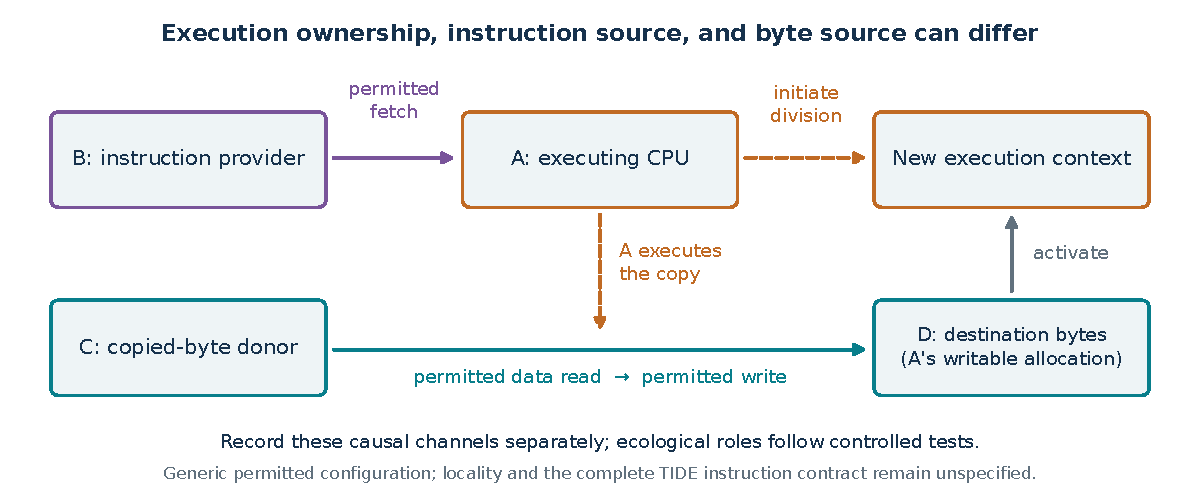
\includegraphics[width=\textwidth]{figures/replication-provenance.pdf}
\caption{Separate causal channels in a generic permitted VM configuration.
A executes instructions supplied by B, copies bytes supplied by C into its
writable allocation D, and initiates division. The diagram extends the
distinctions motivated by Tierra's borrowed copying routines and redirected
copying \citep{Ray1991}; it is neither a recorded three-party Tierra event nor
an approved TIDE contract. Solid colored arrows show instruction/data flow;
dashed arrows show actions of A's execution context.}
\label{fig:provenance}
\end{figure}
Figure~\ref{fig:provenance} explains why byte agreement alone cannot identify
the reproductive mechanism or a unique causal parent.

\subsection{Artificial chemistries and evolving replication reactions}
Artificial chemistries formulate interactions in terms of components and
reaction processes. The important choice is whether a reaction is prescribed
as a fixed transformation or constructed through executable interactions.
Spatial Stringmol is especially relevant to the latter: neighboring strings
bind, execute a reaction, and produce or modify strings
\citep{Hickinbotham2021}. A bound pair is an execution unit, unlike Tierra's
separate CPU ownership. Control flow and copying operations can change how
replication proceeds, rather than changing only a scalar replication rate.

The observed evolution of recognition and copying strategies motivates tests
of functional relationships. It does not imply that a particular ecological
role must survive. Extinction and the later loss of expensive strategies are
part of the evidence. A label such as parasitism should describe consequences
in a stated interaction context, rather than cause those consequences through
special protection, resource transfers, or replacement rules in the kernel.

This distinction suggests a useful experimental progression. First establish
that small fixed programs can perform ordinary self-copy, use another
program's instructions, and redirect copying to a different permitted source.
Then test whether variation produces such pathways and whether their
reproductive effects persist. Expressibility, appearance, and ecological
establishment answer different questions.

\subsection{Origins of replicators and their subsequent spread}
The computational-life experiments of Ag\"uera y Arcas and colleagues examine
replication arising among interacting programs, including conditions without
background mutation \citep{Aguera2024}. Their examples broaden the range of
computational substrates in which replication can arise. They do not remove
the distinction between a first replicator, successful expansion, and the
later evolution of new strategies.

A 2026 BFF follow-up makes that distinction more directly measurable
\citep{Knierim2026}. Under its tested program distributions and detector,
simple random processes can compete with interaction-based searches for
replicators. The detector itself has finite-chain and alignment limitations.
Consequently, origins should be evaluated with explicit candidate replay and
appropriate null searches, while takeover requires a separate population
measurement. These results concern particular short-tape substrates, not a
general theorem about the value of interaction or recombination.

For a supplied-ancestor experiment, the starting question is different:
replication already exists, and the investigator asks what heritable
strategies and dependencies appear afterward. Mixing the two objectives makes
failure difficult to interpret. Failure to find an ancestor in random bytes
need not invalidate a study of evolution after an ancestor; successful spread
of that ancestor does not establish an account of origins.

\subsection{Continuous and neural cellular substrates}
Lenia extends cellular-automata exploration through continuous-valued states,
weighted neighborhoods, and incremental growth rules \citep{Chan2019}. The
2019 study catalogues persistent and moving organizations, while explicitly
leaving self-replication undiscovered in that work. Human-guided exploration
of parameters and initial conditions is therefore distinct from reproduction
and selection within an autonomous population. Later variants must be judged
on their own evidence rather than inheriting either a capability or a
limitation from the original system.

Flow-Lenia introduces mass-conserving dynamics and localized rule parameters
that can interact within one world \citep{Plantec2025}. Directed optimization
and intrinsic evolutionary experiments remain separate parts of the work.
Its measures also expose an interpretive problem: raw activity and
mass-normalized activity can order treatments differently. A parameter vector
used as a species identifier is an operational choice, not an independently
established unit of individuality.

Neural cellular automata address another capability: learning a shared local
rule that develops and repairs a target configuration
\citep{Mordvintsev2020}. The training loss and training distribution are supplied
externally. Distributed deployment and damage recovery demonstrate local
developmental control, not necessarily inherited rule variation or
reproduction-driven evolution during deployment. This separation helps avoid
using ``growth,'' ``regeneration,'' and ``evolution'' interchangeably.

\subsection{External search and AI-assisted discovery}
ASAL uses foundation-model representations to guide searches over artificial-life
simulations \citep{Kumar2025}. Such a search can discover configurations aligned
with a prompt or a chosen novelty/diversity criterion. The representation,
renderer, search algorithm, and evaluation horizon jointly determine which
discoveries are favored. This makes the approach a tool for exploring
substrates, while its evaluator remains outside their internal ecology.

The extended Flow-Lenia exploration study similarly distinguishes
curiosity-driven configuration search from dynamics within a selected
configuration \citep{Michel2026}. Larger or more active simulations require
normalization and longer observation before their apparent complexity can be
interpreted. Search coverage, visually novel trajectories, and endogenous
adaptive innovation should therefore be reported as separate outcomes.

\begin{table}[htbp]
\centering\small
\caption{Selected soft systems compared by their experimental unit and the
claim requiring further evidence. Entries describe the cited studies, not
every implementation or later variant.}
\begin{tabularx}{\textwidth}{@{}>{\raggedright\arraybackslash}p{25mm}YY@{}}
\toprule
System & Main unit or mechanism & What does not follow automatically \\
\midrule
Langton loop & Constructed reproducing pattern & Heritable diversification \\
Evoloop & Interacting reproducing structures & Continuing novelty after convergence \\
Tierra & Executable genome and individual CPU & Unbounded strategy or complexity growth \\
Avida & Configurable digital organisms & Task-independent ecological innovation \\
Stringmol & Executable bound-pair reaction & Universal coexistence or complexity growth \\
BFF & Interacting program tapes & Origin, takeover and innovation being one event \\
Lenia / Flow-Lenia & Continuous local dynamics and, in Flow-Lenia, localized parameters & Morphological diversity identifying evolutionary individuals \\
Neural CA / ASAL & Trained rules or externally searched configurations & Autonomous Darwinian evolution during deployment \\
\bottomrule
\end{tabularx}
\label{tab:soft}
\end{table}
